\documentclass{article}
\pagestyle{empty}
\usepackage{tikz}
\usetikzlibrary{positioning,arrows.meta}
\begin{document}
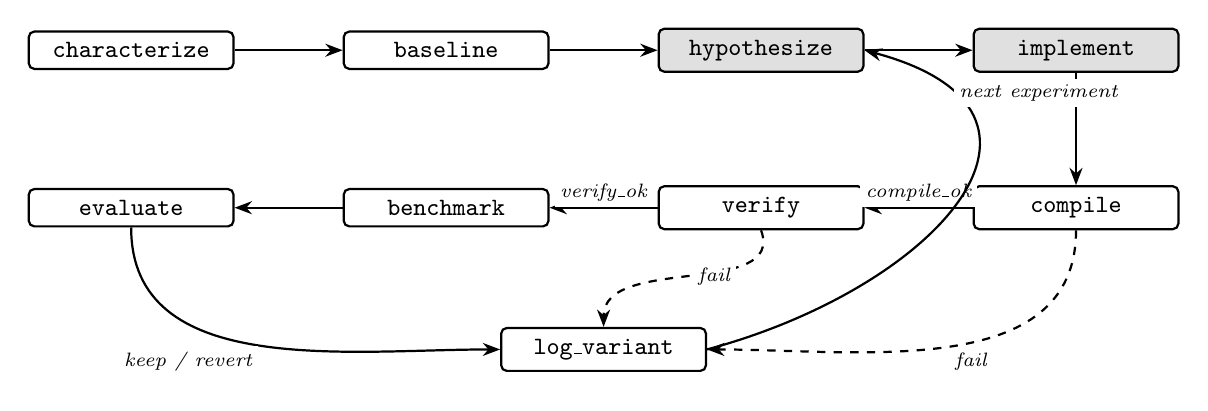
\begin{tikzpicture}[
  >={Stealth[length=2.2mm]},
  state/.style={draw, thick, rounded corners=2pt, font=\small\ttfamily,
    inner xsep=6pt, inner ysep=4pt, minimum width=26mm},
  agent/.style={state, fill=black!12},
  glab/.style={font=\scriptsize\itshape, inner sep=2pt, fill=white}]
\node[state] (ch) at (0,0) {characterize};
\node[state] (ba) at (4.0,0) {baseline};
\node[agent] (hy) at (8.0,0) {hypothesize};
\node[agent] (im) at (12.0,0) {implement};
\node[state] (co) at (12.0,-2.0) {compile};
\node[state] (ve) at (8.0,-2.0) {verify};
\node[state] (be) at (4.0,-2.0) {benchmark};
\node[state] (ev) at (0,-2.0) {evaluate};
\node[state] (lv) at (6.0,-3.8) {log\_variant};
\draw[->, thick] (ch) -- (ba);
\draw[->, thick] (ba) -- (hy);
\draw[->, thick] (hy) -- (im);
\draw[->, thick] (im) -- (co);
\draw[->, thick] (co) -- node[glab, above] {compile\_ok} (ve);
\draw[->, thick] (ve) -- node[glab, above] {verify\_ok} (be);
\draw[->, thick] (be) -- (ev);
\draw[->, thick] (ev.south) to[out=-90, in=180] node[glab, below left] {keep / revert} (lv.west);
\draw[->, thick, dashed] (co.south) to[out=-90, in=0] node[glab, below right] {fail} (lv.east);
\draw[->, thick, dashed] (ve.south) to[out=-70, in=90] node[glab, right] {fail} (lv.north);
\draw[->, thick] (lv.east) to[out=15, in=-15, looseness=1.8]
  node[glab, right, pos=0.82] {next experiment} (hy.east);
\end{tikzpicture}
\end{document}
